\documentclass[helvetica]{seminar} 
\input{xy}
\xyoption{all}
\usepackage{graphicx} 
\usepackage{slidesec} 
\usepackage{url}
\usepackage[framemethod=TikZ]{mdframed}
\usepackage{color}

\long\def\symbolfootnote[#1]#2{\begingroup%
\def\thefootnote{\fnsymbol{footnote}}\footnote[#1]{#2}\endgroup}

% to fix problems making landscape seminar pdfs
% Letter...
\pdfpagewidth=11truein
\pdfpageheight=8.5truein
\pdfhorigin=1truein     % default value(?), but doesn't work without
\pdfvorigin=1truein     % default value(?), but doesn't work without
% A4
%\pdfpagewidth=297truemm % your milage may vary....
%\pdfpageheight=210truemm
%\pdfhorigin=1truein     % default value(?), but doesn't work without
%\pdfvorigin=1truein     % default value(?), but doesn't work without


\renewcommand{\familydefault}{\sfdefault}  
 
\input{seminar.bug} 
\input{seminar.bg2} % See the Seminar bugs list 
 
\slideframe{none} 
 
 
\usepackage{fancyhdr} 
 
% Headers and footers personalization using the `fancyhdr' package 
\fancyhf{} % Clear all fields 
\renewcommand{\headrulewidth}{0mm} 
\renewcommand{\footrulewidth}{0.1mm} 
 
\fancyfoot[L]{\tiny IETF 95} 
\fancyfoot[C]{\tiny DTLS in SDP}
\fancyfoot[R]{\tiny \theslide} 
 
 
% To center horizontally the headers and footers (see seminar.bug) 
\renewcommand{\headwidth}{\textwidth} 

% To adjust the frame length to the header and footer ones 
\autoslidemarginstrue 
\pagestyle{fancy} 
 

\newcommand{\heading}[1]{% 
  \begin{center} 
    \large\bf 
    #1 
  \end{center} 
  \vspace{.4 in}} 



\begin{document}

\begin{slide}
\begin{center}
\vspace{.5 in}
\LARGE{{\bf}DTLS in SDP\\{\small \verb^draft-rescorla-dtls-in-sdp^}}\\
\vspace{.2in}
\large{
\begin{tabular}{c}
Eric Rescorla\\
Mozilla\\
\url{ekr@rtfm.com}
\end{tabular}
}
\end{center}

\end{slide}

\centerslidesfalse 

\begin{slide}
\heading{Tunnelling DTLS in SDP}

\begin{itemize}
\item WebRTC call latency could be better
\item Lots of back and forth
\item Can we improve things
\end{itemize}
\end{slide}

\begin{slide}

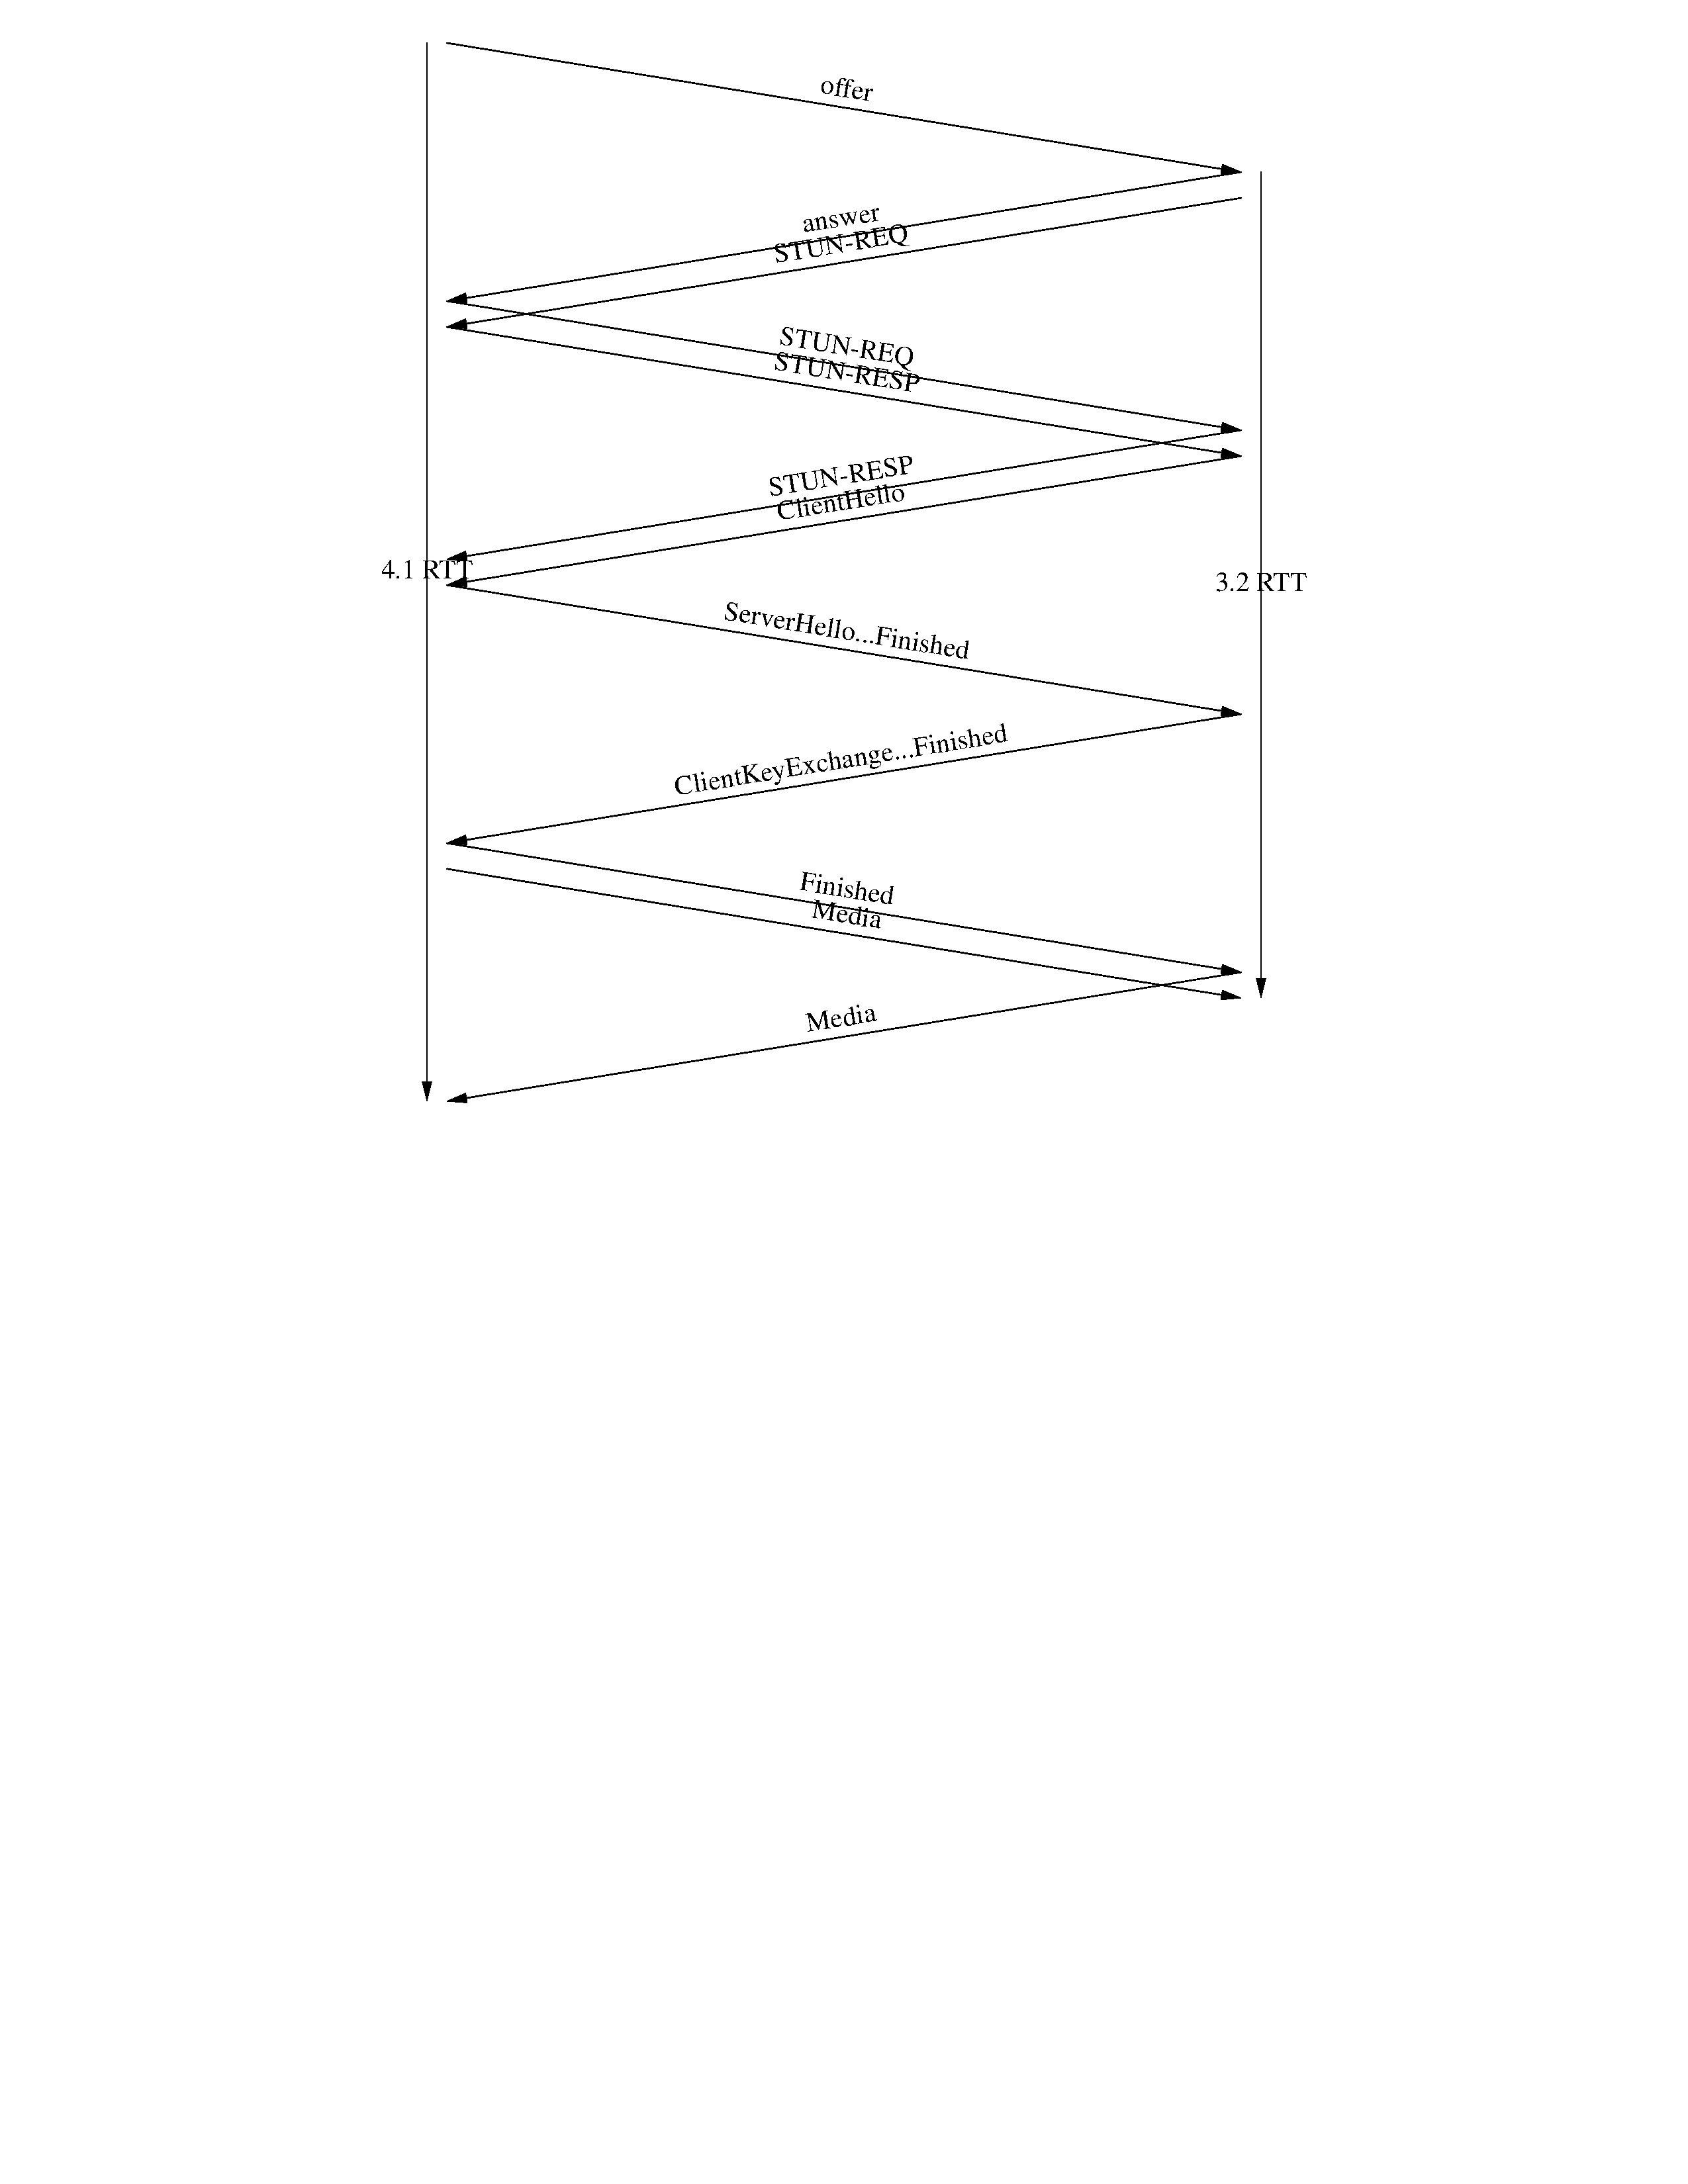
\includegraphics[width=4in]{normal-12}

\end{slide}

\begin{slide}
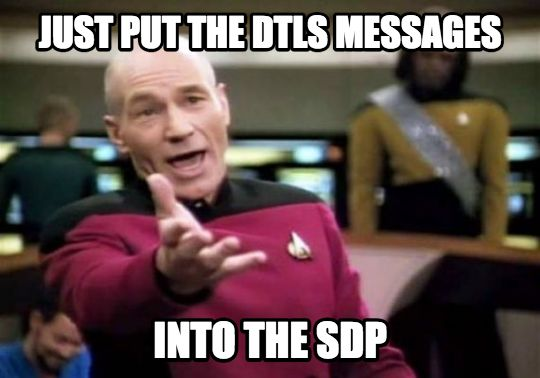
\includegraphics[width=4in]{850871}
\end{slide}


\begin{slide}
\includegraphics[width=4in]{piggybacked-12}
\end{slide}

\begin{slide}
\includegraphics[width=4in]{piggybacked-13}
\end{slide}

\begin{slide}
\includegraphics[width=4in]{piggybacked-13-falsestart}
\end{slide}


\begin{slide}
\heading{What about forking?}

\begin{itemize}
\item ClientHellos can't be processed by two servers
  \begin{itemize}
  \item ... well maybe they can but it seems horrifying
  \end{itemize}
\item Probably need some mechanism for forcing the media plane mode on forks
  \begin{itemize}
  \item Probably easier for WebRTC apps
  \item Ideas for non-WebRTC
  \end{itemize}
\item Maybe some other clever ideas
\end{itemize}
\end{slide}


\begin{slide}
\heading{Security considerations}

\begin{itemize}
\item Needs to be covered by identity
\item Ultimately rooted in the user's key pair
\end{itemize}

\end{slide}


\end{document} 

                